\section{Sausage Gravy}\index{breakfast!sausage gravy}

\begin{center}
Prep Time: 25 min
Total Time: 25 min

\noindent Yield: 12

\vspace{1em}

Source: https://www.foodnetwork.com/recipes/sausage-gravy-2145820
\end{center}

\subsection{Ingredients}
\begin{multicols}{2}
\begin{itemize}
    \item 1 pound breakfast sausage, hot or mild
    \item 1/3 cup all-purpose flour 
    \item 3 to 4 cups whole milk, more to taste 
    \item 1/2 teaspoon seasoned salt 
    \item 2 teaspoons freshly ground black pepper, more to taste 
    \item Biscuits, warmed, for serving
\end{itemize}
\end{multicols}

\subsection{Preparation}
\begin{enumerate}
    \item With your finger, tear small pieces of sausage and add them in a single layer to a large heavy skillet.
        Brown the sausage over medium-high heat until no longer pink. Reduce the heat to medium-low.
    \item Sprinkle on half the flour and stir so that the sausage soaks it all up, then add more little by little.
        Stir it around and cook it for another minute or so, then pour in the milk, stirring constantly.
    \item Cook the gravy, stirring frequently, until it thickens.
        (This may take a good 10 to 12 minutes.)
        Sprinkle in the seasoned salt and pepper and continue cooking until very thick and luscious.
        If it gets too thick too soon, just splash in another 1/2 cup of milk or more if needed.
        Taste and adjust the seasoning.
    \item Spoon the sausage gravy over warm biscuits and serve immediately!
\end{enumerate}

\begin{figure}[h!]
    \centering
    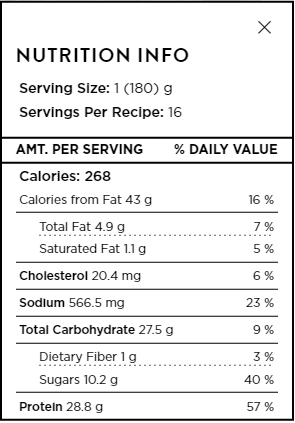
\includegraphics[width=.25\textwidth]{img/crock-pot-shredded-venison-nutrition.png}
    \caption{Nutrition information for crock pot shredded venison.}
    \label{fig:crock-pot-shredded-venison}
\end{figure}
